%%%%%%%%%%%%%%%%%%%%%%%%%%%%%%%%%%%%%%%%%
% Journal Article
% LaTeX Template
% Version 1.4 (15/5/16)
%
% This template has been downloaded from:
% http://www.LaTeXTemplates.com
%
% Original author:
% Frits Wenneker (http://www.howtotex.com) with extensive modifications by
% Vel (vel@LaTeXTemplates.com)
%
% License:
% CC BY-NC-SA 3.0 (http://creativecommons.org/licenses/by-nc-sa/3.0/)
%
%%%%%%%%%%%%%%%%%%%%%%%%%%%%%%%%%%%%%%%%%

%----------------------------------------------------------------------------------------
%	PACKAGES AND OTHER DOCUMENT CONFIGURATIONS
%----------------------------------------------------------------------------------------

\documentclass{article}

\usepackage{blindtext} % Package to generate dummy text throughout this template 

\usepackage[sc]{mathpazo} % Use the Palatino font
\usepackage[T1]{fontenc} % Use 8-bit encoding that has 256 glyphs
\linespread{1.05} % Line spacing - Palatino needs more space between lines
\usepackage{microtype} % Slightly tweak font spacing for aesthetics

\usepackage[english]{babel} % Language hyphenation and typographical rules

\usepackage[hmarginratio=1:1,top=32mm,columnsep=20pt]{geometry} % Document margins
\usepackage[hang, small,labelfont=bf,up,textfont=it,up]{caption} % Custom captions under/above floats in tables or figures
\usepackage{booktabs} % Horizontal rules in tables

\usepackage{lettrine} % The lettrine is the first enlarged letter at the beginning of the text

\usepackage{enumitem} % Customized lists
\setlist[itemize]{noitemsep} % Make itemize lists more compact

\usepackage{abstract} % Allows abstract customization
\renewcommand{\abstractnamefont}{\normalfont\bfseries} % Set the "Abstract" text to bold
\renewcommand{\abstracttextfont}{\normalfont\small\itshape} % Set the abstract itself to small italic text

\usepackage{titlesec} % Allows customization of titles
\renewcommand\thesection{\Roman{section}} % Roman numerals for the sections
\renewcommand\thesubsection{\roman{subsection}} % roman numerals for subsections
\titleformat{\section}[block]{\large\scshape\centering}{\thesection.}{1em}{} % Change the look of the section titles
\titleformat{\subsection}[block]{\large}{\thesubsection.}{1em}{} % Change the look of the section titles

\usepackage{fancyhdr} % Headers and footers
\pagestyle{fancy} % All pages have headers and footers
\fancyhead{} % Blank out the default header
\fancyfoot{} % Blank out the default footer
\fancyhead[C]{\textit{Plasmodium vivax} thick blood image masks development} % Custom header text
\fancyfoot[RO,LE]{\thepage} % Custom footer text

\usepackage{titling} % Customizing the title section

\usepackage{hyperref} % For hyperlinks in the PDF
\usepackage{graphicx}
\usepackage{multirow}
\usepackage{amsmath}
%----------------------------------------------------------------------------------------
%	TITLE SECTION
%----------------------------------------------------------------------------------------

\setlength{\droptitle}{-4\baselineskip} % Move the title up

\pretitle{\begin{center}\Huge\bfseries} % Article title formatting
\posttitle{\end{center}} % Article title closing formatting
\title{\textit{Plasmodium vivax} thick blood image masks development} % Article title
\author{%
\textsc{Jorge Augusto Balsells Orellana} \\[1ex] % Your name
\and
\textsc{Erick Wilfredo D\'{i}az Saborio} \\[1ex] % Second author's name
\and 
\textsc{Sofia Maribel Soberanis Lopez} \\[1ex] % Second author's name
\and 
\textsc{Cindy Carolina Rocio Villalobos Morales} \\[1ex] % Second author's name
\and 
\textsc{Hans Iv\'{o} Roche Villagr\'{a}n} \\[1ex] % Second author's name
\normalsize University of San Carlos de Guatemala \\ % Your institution
}
\date{\today} % Leave empty to omit a date
\renewcommand{\maketitlehookd}

%----------------------------------------------------------------------------------------

\begin{document}

% Print the title
\maketitle

%----------------------------------------------------------------------------------------
%	ARTICLE CONTENTS
%----------------------------------------------------------------------------------------

\section{Abstract}

Malaria is a disease transmitted by the bite of the female mosquito of the genus \textit{Anoppheles} infected by protozoa of the genus \textit{Plasmodium}, which is obligate intracellular parasites. \textit{P. vivax} is the sole cause of the disease in Guatemala and currently focuses on the departments of Escuintla, Alta Verapaz, Izabal and Suchitepéquez. The signs and symptoms caused by \textit{P. vivax} infections are fever and fatigue, this \textit{Plasmodium} has the peculiarity of maintaining "dormant" forms (hypnozoites) in the liver, which gives the possibility of recurrence of the disease. In addition, it may present complications due to splenomegaly, rupture of the organ with concomitant internal bleeding (Pan American Health Organization, 2017).

In Guatemala, the techniques currently used for the diagnosis of \textit{P. vivax} are the microscopic examination of the protozoan through two types of blood films: thick blood smear and peripheral smear (National Health Laboratory, 2017). However, this type of diagnosis has some disadvantages: trained and experienced microscopist personnel to identify and quantify the parasite in the thick drop (gold standard) and peripheral rub given that the parasite can be confused with platelets, precipitate, white blood cells or artifacts; high workload for staff depending on the area in which the disease is concentrated; high estimated time in observation of blood films, on average a trained person observes a thick blood film for 10 to 20 minutes, in endemic areas a health center can receive between 200 and 300 weekly blood films; Ocular fatigue, usually is the most influential factor in an incorrect diagnosis, this is due to long periods of time observing samples through the microscope.

This investigation objective, is to design a raw tick blood images, data processing pipeline that generates a clean dataset, that can be used for training models like convolutional neural networks (CNN) models. In order to train these models is required a good dataset, that have been quantitatively measured for an objective, in this case detect malaria. Our initial data exploration analysis on the images shows that, the images have differents sizes and the image is not centered (\textbf{Supplementary Fig 1}). The code of this initial data exploration analysis can be found at \url{https://github.com/ErickDiaz/bioinformatic_thesis_project/blob/master/code/data-exploration/data_exploration.ipynb}.

%----------------------------------------------------------------------------------------
%	METHODS
%----------------------------------------------------------------------------------------

\section{Methods}

This work pretends to  find patterns in these biological data and detect the malaria parasite \textit{P. vivax}, using the following techniques. 
\begin{itemize}
\item Edge detection
\item Sobel Filters
\item Convolution FIlters
\item Histograms of image value distribution, and use the cumulative distribution function for finding the frequency of a given range of pixel intensity occurrence.
\end{itemize}
In order to quantify how good the filters are, we will use two cost functions that will measure how is our pipeline filtering the parasite. The cost function will measure the mask generated by the pipeline against manually generated masks by our team, using an open source tool called LabelImg.The goal of the data pipeline is to minimize the values of the cost functions.
\begin{itemize}
\item Mean Absolute error: Calculate the similarity, because we want to measure if there is a difference between two images after applying the masks.
\item The intersection of the union(IOU): Measure the total number of shared pixels after applying the masks. \\  \begin{equation*}
  IOU = \frac{I_1 \cup I_2}{I_1 \cap I_2}
\end{equation*}
\end{itemize}


%----------------------------------------------------------------------------------------
%	RESOURCES
%----------------------------------------------------------------------------------------
\section{Resources}

% Please add the following required packages to your document preamble:
% \usepackage{multirow}
\begin{table}[hbt!]
\begin{tabular}{llll}
\cline{1-3}
\multicolumn{3}{|c|}{Resources}                                                                                                                                                                                                                                                                                                                                                                                                                                    &  \\ \cline{1-3}
\multicolumn{1}{|l|}{Material}                                                                                                      & \multicolumn{1}{l|}{Finantial}                                                                             & \multicolumn{1}{l|}{Human}                                                                                                                                                                                      &  \\ \cline{1-3}
\multicolumn{1}{|l|}{tick blood images}                                                                                             & \multicolumn{1}{l|}{\begin{tabular}[c]{@{}l@{}}AWS, \\ Instance c5.4xLarge: \\ 0.68 USD/Hora\end{tabular}} & \multicolumn{1}{l|}{\multirow{4}{*}{\begin{tabular}[c]{@{}l@{}}Jorge Balsells Orellana, \\ Erick Diaz Saborio, \\ Sofia Soberanis Lopez,\\ Cindy Villalobos Morales, \\ Hans Ivó Roche Villagrán\end{tabular}}} &  \\ \cline{1-2}
\multicolumn{1}{|l|}{\begin{tabular}[c]{@{}l@{}}Manual Bounding Boxes tooll : \\ https://github.com/tzutalin/labelImg\end{tabular}} & \multicolumn{1}{l|}{\$ 0.00}                                                                               & \multicolumn{1}{l|}{}                                                                                                                                                                                           &  \\ \cline{1-2}
\multicolumn{1}{|l|}{Python}                                                                                                        & \multicolumn{1}{l|}{\$ 0.00}                                                                               & \multicolumn{1}{l|}{}                                                                                                                                                                                           &  \\ \cline{1-2}
\multicolumn{1}{|l|}{GitHub}                                                                                                        & \multicolumn{1}{l|}{\$ 0.00}                                                                               & \multicolumn{1}{l|}{}                                                                                                                                                                                           &  \\ \cline{1-3}
                                                                                                                                    &                                                                                                            &                                                                                                                                                                                                                 & 
\end{tabular}
\end{table}

%----------------------------------------------------------------------------------------
%	RESULTS AND EXPECTED IMPACT
%----------------------------------------------------------------------------------------

\section{Results and expected impact}


\begin{itemize}
\item Create a raw tick blood image processing pipeline that generates a database of treated images, classified by positive and negative samples. For each positive sample a set of masks that will indicate the location of the parasites. The purpose will be its use to experiment with different models of neural networks, in order to detect positive samples and the count of parasites in the sample.
\item Contribute to the scientific advance of bioinformatics in Guatemala by sharing the dataset of malaria blood samples in Kaggle. This website is a community of data scientists, in which users can publish datasets, code of artificial intelligence models called kernels and discussion forums. Once a kernel is publish it allows users to fork this allows collaborative programming, also vote for a kernel and add comments.
\end{itemize}

%----------------------------------------------------------------------------------------
%	REFERENCE LIST
%----------------------------------------------------------------------------------------
\section{References}
\begin{itemize}
\item Clinically applicable deep learning for diagnosis and referral in retinal”(Pearse A. Keane, 2018)
\item Deep learning enabled multi-wavelength spatial coherence microscope for the classification of malaria-infected stages with limited labelled data size (Neeru Singla and Vishal Srivastava, 2019)
\item Purwar, Y., Shah, S. Clarke, G. \& Muehlenbachs A. (2011). Automated and unsupervised detection of malarial parasites in microscopic images. Malaria Journal 10 (364).
\item Organización panamericana de la Salud. (2017). Marco para la eliminación de la malaria. Washington: Organización Panamericana de la Salud.
\item Laboratorio Nacional de Salud. (2ª Ed.). (2017). Manual de normas y procedimientos de laboratorio para el diagnóstico de malaria. Guatemala: Ministerio de Salud Pública y Asistencia Social, Dirección de Regulación, Vigilancia y Control de la Salud, Laboratorio Nacional de Salud.
\item Lopez, E. (2019). Ops/oms Guatemala - Guatemala Avanza En La Lucha Contra La Malaria. Recuperado de: \url{https://www.paho.org/gut/index.php?option=com_content&view=article&id=1220%3Aguatemala-avanza-en-la-lucha-contra-la-malaria&Itemid=441}


\end{itemize}






%----------------------------------------------------------------------------------------
%	Supplementary Information
%----------------------------------------------------------------------------------------
\section{Supplementary Information}
\subsection{Supplementary Figures}

\begin{figure}[hbt!]
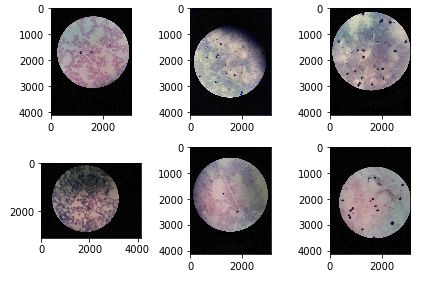
\includegraphics[height=9cm, width=13cm]{image_samples.png}
\caption{Example of images in the raw dataset.}
\label{fig:img_samples}
\end{figure}



%----------------------------------------------------------------------------------------

\end{document}
